\chapter{超新星遗迹和磁流体相关理论}
\label{Theory}

\section{超新星遗迹激波加速和宇宙线}
\label{TheoryDSACR}
二战结束后,很多用于军事的射电观测设备和技术被应用于天文探索,而这段时间观测发现银河系内
存在很多非热射电源。
\citet{1953AZh....30...15S}首次提出这些非热辐射源自于过去爆发却未被看到的超新星爆发
产生的残骸,而辐射机制就是同步辐射。
这一猜测随着观测的增多逐步得到证实,直到今天,射电观测仍然是证认SNR的重要手段,而截至
目前,我们已经观测到近300个SNR\citep{2014BASI...42...47G}。

可是,同步辐射产生SNR的非热谱有一个前提,就是辐射电子是相对论化且幂律分布的
\citep{1970ranp.book.....P}。
\citet{Fermi1949}提出的宇宙线加速机制刚好使得电子可以满足这一前提,同时也提到了超新星
爆发或者SNR演化或许会引起这样的加速,\citet{1953AZh....30...15S}也是以此为依据提出同步
辐射机制产生SNR中的射电辐射。
而Fermi其实更多是想解释观测到的宇宙线能谱,因为当时逐渐受到关注的宇宙线观测显示其能谱是
幂律谱,这就需要一个加速机制解释这件事,所以他只是提出了一个能产生幂律谱的机制,并没有
深入阐述这个机制如何在SNR中起作用。
这主要是个将磁化云块作为磁镜的机制,因为粒子接近云块加速远离云块减速,所以互相抵消,结果
加速效率与云块的速度$\mu$和粒子的速度$\nu$的二次方成正比,我们称之为费米二阶加速机制。
很快,有人注意到这个机制的加速效率过低,不足以解释观测结果,并尝试寻找更高效的加速机制。
同时,人们意识到,强激波中的加速可以实现只有粒子接近云块的加速过程,而没有离开云块的减速
过程,这样加速效率与云块的速度$\mu$和粒子的速度$\nu$的一次方成正比,我们称之为费米一阶
加速机制,又称扩散激波加速机制(Diffusive Shock Acceleration, DSA)
\citep{1977ICRC...11..132A,1977SPhD...22..327K,Bell1978,Blandford1978}。
通常,我们所说的费米加速机制主要就是指费米一阶加速,也就是DSA。

\subsection{扩散激波加速机制}
我们知道,物体在介质中进行超音速运动就会形成激波。
而在SNR中,所谓的介质就是ISM,而超音速运动的物体就是超新星爆发的抛射物。
抛射物挤压ISM,导致ISM在抛射物前方堆积,形成激波面。
也就是说,抛射物与激波面虽然很近,但是还有一定距离,类似于超音速飞机与其前方激波的关系。
通常理想气体介质中的声速$c_s$可以由$c_s=\sqrt{\gamma kT/m}$表示,其中$\gamma$是绝热系数,
$k$是玻尔兹曼常数,$T$是温度,$m$是单个粒子质量。
通常我们认为介质中主要由质子组成,那么$m$就采用质子质量,有时要考虑He核,那就使用平均原子
权重得到约化质量作为$m$。
假设介质组成全部是质子,可得$c_s\approx 0.1\sqrt{T/K}$ \kms 。
超新星抛射物马赫数为$M=v/c_s$,如果$M\gg 1$则为强激波。
超新星抛射物速度$v$可超过10000 \kms ,而即使介质温度达到10$^6$K,$c_s$也只有100 \kms 。
所以,即使没有介质冷的条件,超新星遗迹的激波也肯定是强激波。
此外,要提到的是,通常大质量恒星星风速度可接近1000 \kms,有时也可以视作强激波。

\begin{figure*}
    \centering
    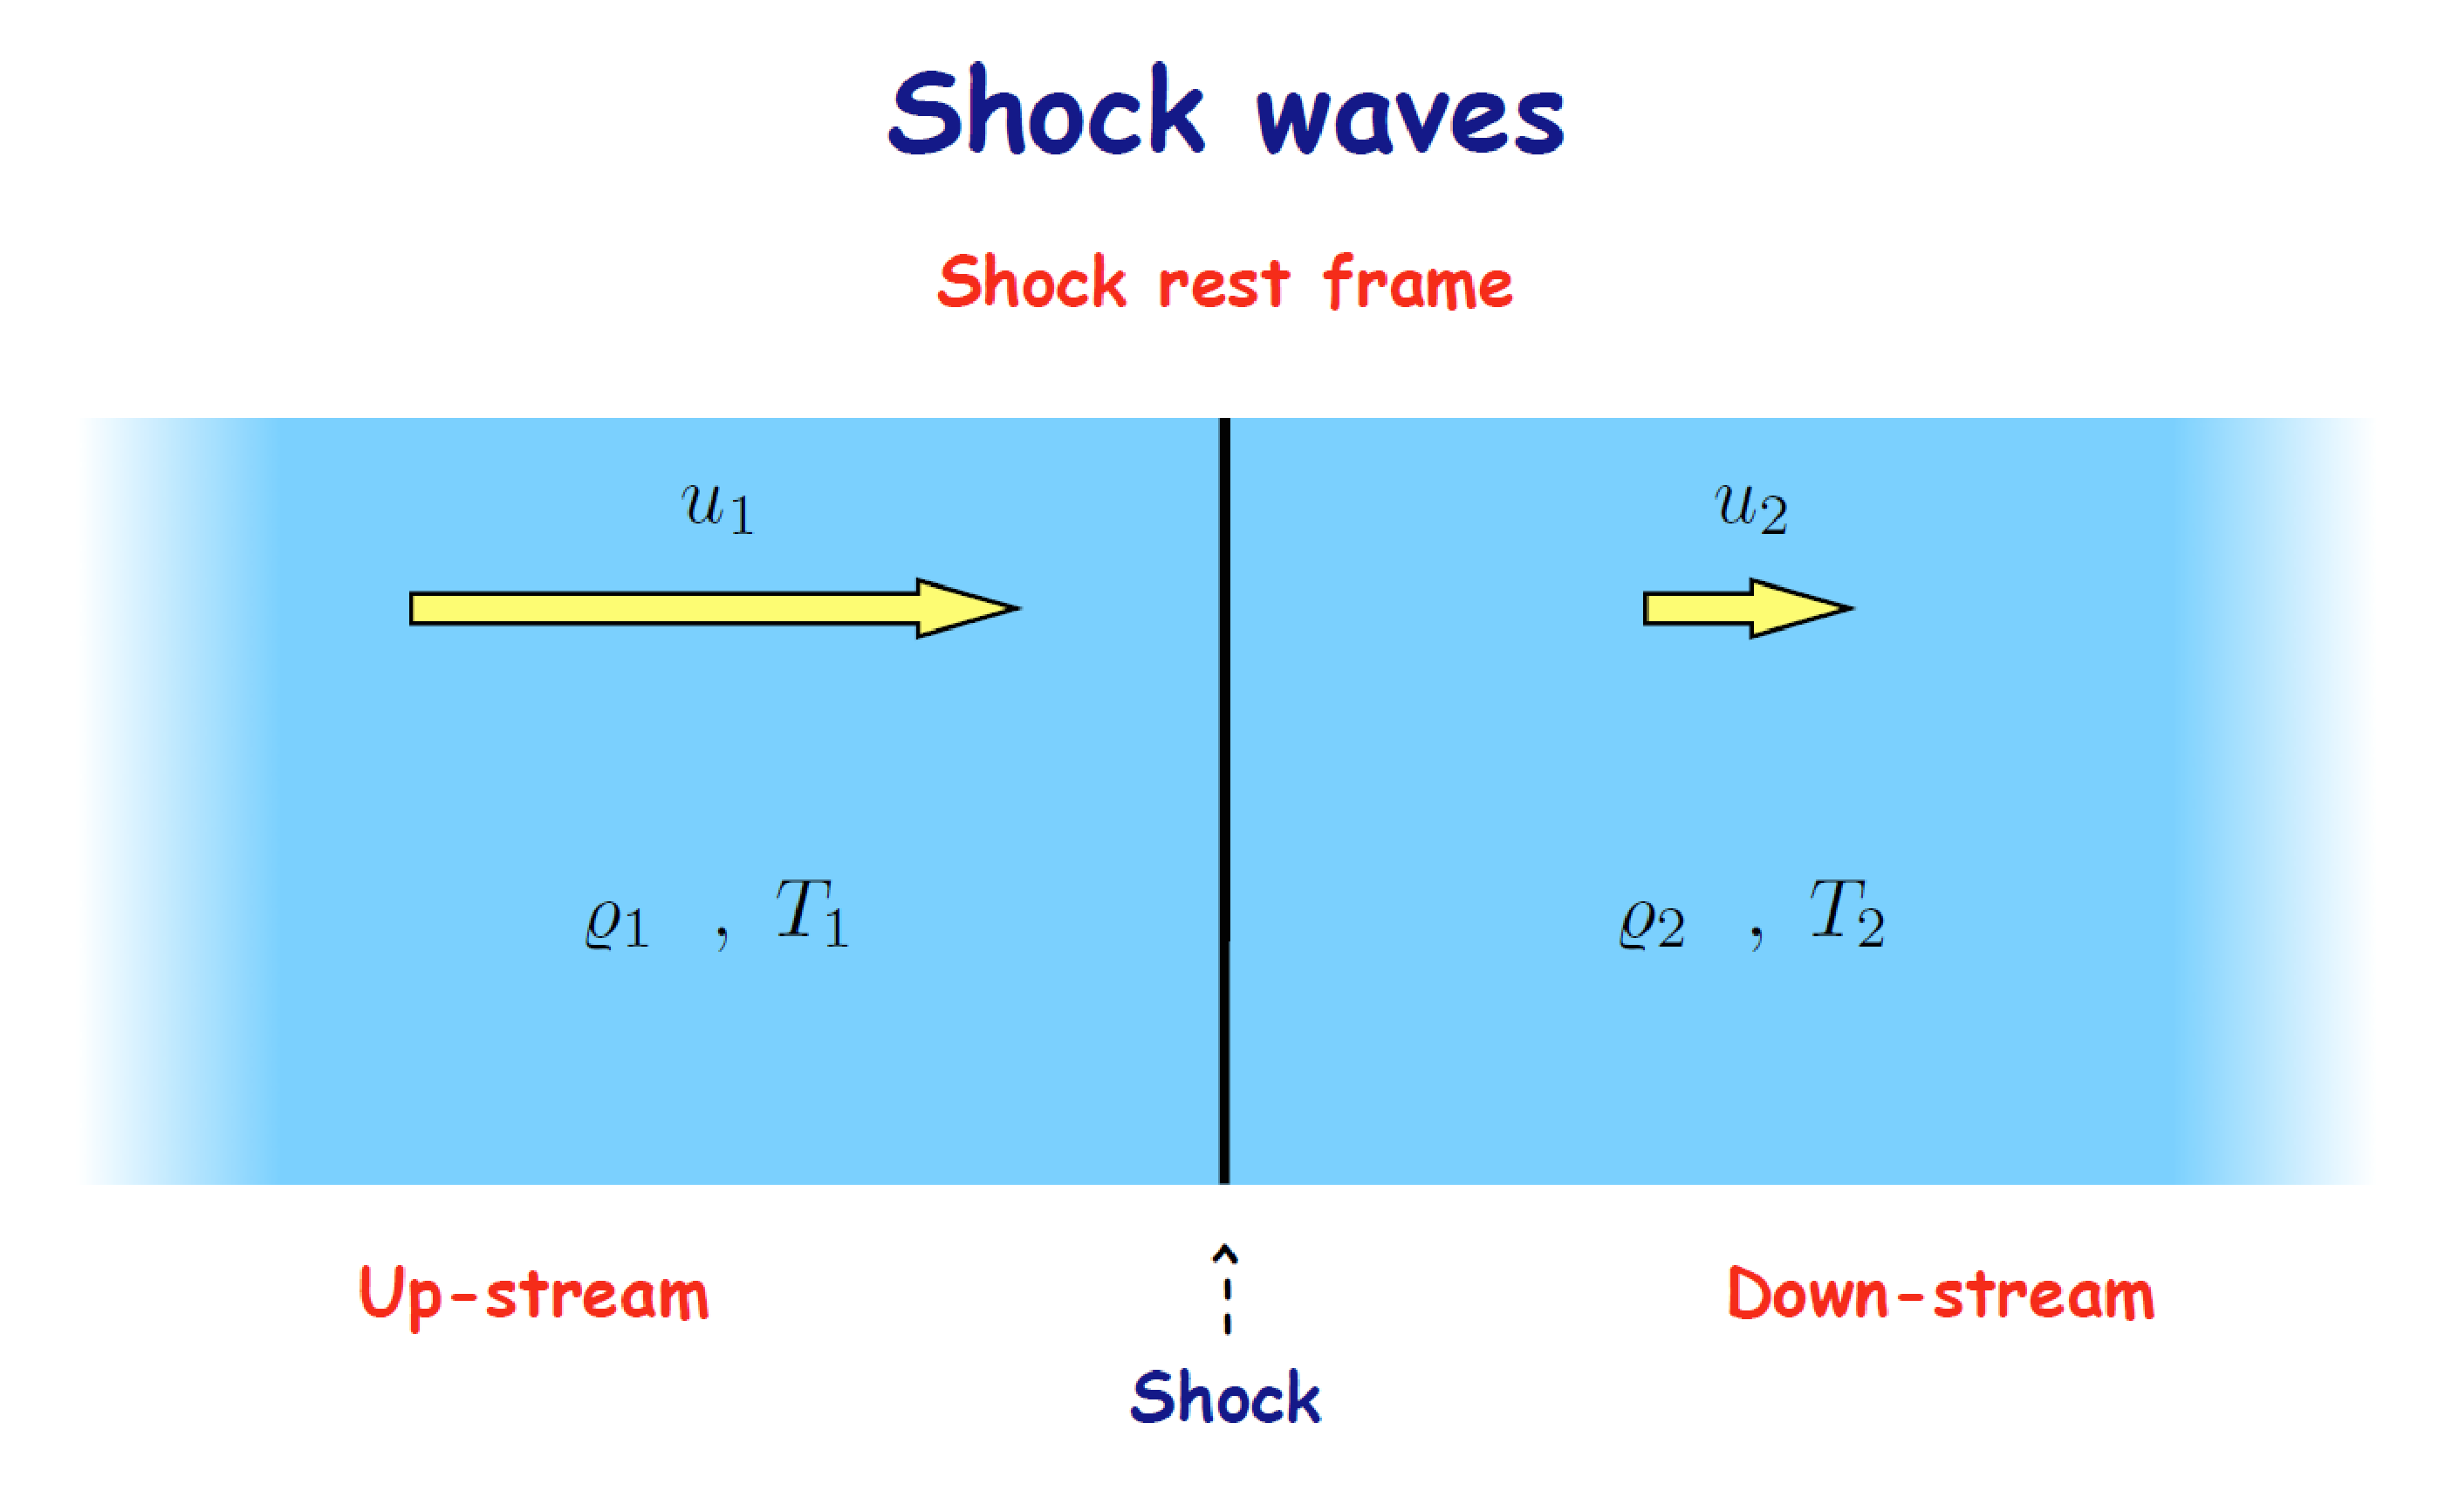
\includegraphics[width=0.9\textwidth]{shock.eps}
    \caption{激波面静止参考系上下游的状态,图片来自Dr. Stefano Gabici。}
\label{fig:shock}
\end{figure*}

而激波的重要特征之一就是,激波面分割开的上游和下游物理量差异很大,或者称为激波面不连续性。
取激波面为静止参考系,运动朝向激波面的为上游,速度、密度、温度为$\mu_1$、$\rho_1$、$T_1$,
远离激波面的为下游,速度、密度、温度为$\mu_2$、$\rho_2$、$T_2$,如图~\ref{fig:shock}。
要注意,这里并没有抛射物混入,所以上下游其实都是原本就存在的ISM或者CSM,因而应该满足质量
守恒$\rho_1\mu_1=\rho_2\mu_2$,这里我们定义压缩比$r=\rho_2/\rho_1=\mu_1/\mu_2$。
而这里的动量守恒可粗略写为$\rho_1\mu_1^2=\rho_2\mu_2^2$,我们知道压强其实就是运动粒子
的动量造成的,这里的动量其实就是动压。
而热压在这里其实也是不可忽略的,所以准确的动量守恒方程应该为
$\rho_1\mu_1^2+p_1=\rho_2\mu_2^2+p_2$。
这里我们忽略了磁场,而遗迹当中磁压其实也很重要,考虑进来的话可得
$\rho_1\mu_1^2+p_1+B_1^2/2=\rho_2\mu_2^2+p2+B_2^2/2$。
不过在这一节的讨论中,我们不考虑磁压,更多关于磁压的讨论请见章节~\ref{ThoryMHD}。
此外,我们这里的讨论都使用高斯单位制,具体计算时需要注意。

又因为$c_{s}^{2}=\gamma p/\rho}$将不考虑磁压的动量守恒方程改写为

\begin{equation}
  \begin{aligned}
    \rho_{1} u_{1}^{2}\left(1+\frac{p_{1}}{\rho_{1} u_{1}^{2}}\right)=
    \rho_{1} u_{1}^{2}\left(1+\frac{c_{s, 1}^{2}}{\gamma u_{1}^{2}}\right)=
    \rho_{1} u_{1}^{2}\left(1+\frac{1}{\gamma M_1^{2}}\right).
  \end{aligned}
\end{equation}

假设在国际标准参考系中(International Celestial Reference Frame,ICRF)激波上游介质在SNR
演化时标内可看作是静止的,我们在激波面的静止系中看到的$\mu_1$其实就是激波面本身的速度,
$M_1$与$M$其实是一个量。
而$M\gg 1$,所以近似得$\rho_1\mu_1^2+p_1=\rho_1\mu_1^2$,
也就是$\rho_1\mu_1^2=\rho_2\mu_2^2+p_2$,两侧除以$\rho_2\mu_2^2$可得

\begin{equation}
    \begin{aligned}
       \frac{u_{1}}{u_{2}}=1+\frac{p_{2}}{\rho_{2} u_{2}^{2}}
       =1+\frac{1}{\gamma M_{2}^{2}} \ ,
    \end{aligned}
\end{equation}

如果取$\gamma$=5/3,可得$r=1+3/(5 M_{2}^{2})$。

能量守恒方程类似,$0.5\rho_1\mu_1^3+\rho_1\mu_1\epsilon_1=
0.5\rho_2\mu_2^3+\rho_2\mu_2\epsilon_2$,其中$\rho\epsilon$代表相对应的内能密度。
理想气体中,$\epsilon=p/\rho/(\gamma-1)$,所以可得:

\begin{equation}
    \begin{aligned}
      \dfrac{1}{2}\rho_1\mu_1^3+\dfrac{1}{\gamma-1}p_1\mu_1=
      \dfrac{1}{2}\rho_2\mu_2^3+\dfrac{1}{\gamma-1}p_2\mu_2\ ,
    \end{aligned}
\end{equation}

同样因为$M_1\gg 1$,所以两侧除以$0.5\rho_2\mu_2^3$,可得$r^2=1+3/(M_{2}^{2})$。
与$r=1+3/(5 M_{2}^{2})$联立解方程组可得$r=4, M_{2}^{2}=0.2$。

激波上游主要是介质构成,而激波下游主要是受到SNR激波影响。
根据这个推导,我们可以通过介质和激波的性质,估计受到影响后的介质性质。
比如:
\begin{equation}
    \begin{aligned}
      \frac{1}{5}=M_{2}^{2}=\frac{\mu_{2}^{2}}{c_{s, 2}^{2}}=
      \frac{\mu_{1}^{2}}{16 c_{s, 2}^{2}}=\frac{m \mu_{1}^{2}}{16 \gamma k T_{2}}\ ,
    \end{aligned}
\end{equation}
因而可得$k T_{2}=3/16 m \mu_{1}^{2}$。
如果取质量比[H/He]=3,则可得
这是一个很重要的推论,可以帮助我们理解很多SNR演化的细节。
首先,记得我们在章节~\label{SNRintro}提到过

\section{磁流体模拟基础}
\label{ThoryMHD}
